\documentclass[1p]{elsarticle_modified}
%\bibliographystyle{elsarticle-num}

%\usepackage[colorlinks]{hyperref}
%\usepackage{abbrmath_seonhwa} %\Abb, \Ascr, \Acal ,\Abf, \Afrak
\usepackage{amsfonts}
\usepackage{amssymb}
\usepackage{amsmath}
\usepackage{amsthm}
\usepackage{scalefnt}
\usepackage{amsbsy}
\usepackage{kotex}
\usepackage{caption}
\usepackage{subfig}
\usepackage{color}
\usepackage{graphicx}
\usepackage{xcolor} %% white, black, red, green, blue, cyan, magenta, yellow
\usepackage{float}
\usepackage{setspace}
\usepackage{hyperref}

\usepackage{tikz}
\usetikzlibrary{arrows}

\usepackage{multirow}
\usepackage{array} % fixed length table
\usepackage{hhline}

%%%%%%%%%%%%%%%%%%%%%
\makeatletter
\renewcommand*\env@matrix[1][\arraystretch]{%
	\edef\arraystretch{#1}%
	\hskip -\arraycolsep
	\let\@ifnextchar\new@ifnextchar
	\array{*\c@MaxMatrixCols c}}
\makeatother %https://tex.stackexchange.com/questions/14071/how-can-i-increase-the-line-spacing-in-a-matrix
%%%%%%%%%%%%%%%

\usepackage[normalem]{ulem}

\newcommand{\msout}[1]{\ifmmode\text{\sout{\ensuremath{#1}}}\else\sout{#1}\fi}
%SOURCE: \msout is \stkout macro in https://tex.stackexchange.com/questions/20609/strikeout-in-math-mode

\newcommand{\cancel}[1]{
	\ifmmode
	{\color{red}\msout{#1}}
	\else
	{\color{red}\sout{#1}}
	\fi
}

\newcommand{\add}[1]{
	{\color{blue}\uwave{#1}}
}

\newcommand{\replace}[2]{
	\ifmmode
	{\color{red}\msout{#1}}{\color{blue}\uwave{#2}}
	\else
	{\color{red}\sout{#1}}{\color{blue}\uwave{#2}}
	\fi
}

\newcommand{\Sol}{\mathcal{S}} %segment
\newcommand{\D}{D} %diagram
\newcommand{\A}{\mathcal{A}} %arc


%%%%%%%%%%%%%%%%%%%%%%%%%%%%%5 test

\def\sl{\operatorname{\textup{SL}}(2,\Cbb)}
\def\psl{\operatorname{\textup{PSL}}(2,\Cbb)}
\def\quan{\mkern 1mu \triangleright \mkern 1mu}

\theoremstyle{definition}
\newtheorem{thm}{Theorem}[section]
\newtheorem{prop}[thm]{Proposition}
\newtheorem{lem}[thm]{Lemma}
\newtheorem{ques}[thm]{Question}
\newtheorem{cor}[thm]{Corollary}
\newtheorem{defn}[thm]{Definition}
\newtheorem{exam}[thm]{Example}
\newtheorem{rmk}[thm]{Remark}
\newtheorem{alg}[thm]{Algorithm}

\newcommand{\I}{\sqrt{-1}}
\begin{document}

%\begin{frontmatter}
%
%\title{Boundary parabolic representations of knots up to 8 crossings}
%
%%% Group authors per affiliation:
%\author{Yunhi Cho} 
%\address{Department of Mathematics, University of Seoul, Seoul, Korea}
%\ead{yhcho@uos.ac.kr}
%
%
%\author{Seonhwa Kim} %\fnref{s_kim}}
%\address{Center for Geometry and Physics, Institute for Basic Science, Pohang, 37673, Korea}
%\ead{ryeona17@ibs.re.kr}
%
%\author{Hyuk Kim}
%\address{Department of Mathematical Sciences, Seoul National University, Seoul 08826, Korea}
%\ead{hyukkim@snu.ac.kr}
%
%\author{Seokbeom Yoon}
%\address{Department of Mathematical Sciences, Seoul National University, Seoul, 08826,  Korea}
%\ead{sbyoon15@snu.ac.kr}
%
%\begin{abstract}
%We find all boundary parabolic representation of knots up to 8 crossings.
%
%\end{abstract}
%\begin{keyword}
%    \MSC[2010] 57M25 
%\end{keyword}
%
%\end{frontmatter}

%\linenumbers
%\tableofcontents
%
\newcommand\colored[1]{\textcolor{white}{\rule[-0.35ex]{0.8em}{1.4ex}}\kern-0.8em\color{red} #1}%
%\newcommand\colored[1]{\textcolor{white}{ #1}\kern-2.17ex	\textcolor{white}{ #1}\kern-1.81ex	\textcolor{white}{ #1}\kern-2.15ex\color{red}#1	}

{\Large $\underline{12n_{0184}~(K12n_{0184})}$}

\setlength{\tabcolsep}{10pt}
\renewcommand{\arraystretch}{1.6}
\vspace{1cm}\begin{tabular}{m{100pt}>{\centering\arraybackslash}m{274pt}}
\multirow{5}{120pt}{
	\centering
	\includegraphics[width=112pt]{../../../GIT/diagram.site/Diagrams/png/2273_12n_0184.png}\\
\ \ \ A knot diagram\footnotemark}&
\allowdisplaybreaks
\textbf{Linearized knot diagam} \\
\cline{2-2}
 &
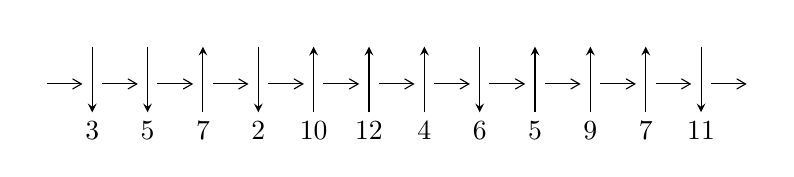
\begin{tikzpicture}[x=20pt, y=17pt]
	% nodes
	\node (C0) at (0, 0) {};
	\node (C1) at (1, 0) {};
	\node (C1U) at (1, +1) {};
	\node (C1D) at (1, -1) {3};

	\node (C2) at (2, 0) {};
	\node (C2U) at (2, +1) {};
	\node (C2D) at (2, -1) {5};

	\node (C3) at (3, 0) {};
	\node (C3U) at (3, +1) {};
	\node (C3D) at (3, -1) {7};

	\node (C4) at (4, 0) {};
	\node (C4U) at (4, +1) {};
	\node (C4D) at (4, -1) {2};

	\node (C5) at (5, 0) {};
	\node (C5U) at (5, +1) {};
	\node (C5D) at (5, -1) {10};

	\node (C6) at (6, 0) {};
	\node (C6U) at (6, +1) {};
	\node (C6D) at (6, -1) {12};

	\node (C7) at (7, 0) {};
	\node (C7U) at (7, +1) {};
	\node (C7D) at (7, -1) {4};

	\node (C8) at (8, 0) {};
	\node (C8U) at (8, +1) {};
	\node (C8D) at (8, -1) {6};

	\node (C9) at (9, 0) {};
	\node (C9U) at (9, +1) {};
	\node (C9D) at (9, -1) {5};

	\node (C10) at (10, 0) {};
	\node (C10U) at (10, +1) {};
	\node (C10D) at (10, -1) {9};

	\node (C11) at (11, 0) {};
	\node (C11U) at (11, +1) {};
	\node (C11D) at (11, -1) {7};

	\node (C12) at (12, 0) {};
	\node (C12U) at (12, +1) {};
	\node (C12D) at (12, -1) {11};
	\node (C13) at (13, 0) {};

	% arrows
	\draw[->,>={angle 60}]
	(C0) edge (C1) (C1) edge (C2) (C2) edge (C3) (C3) edge (C4) (C4) edge (C5) (C5) edge (C6) (C6) edge (C7) (C7) edge (C8) (C8) edge (C9) (C9) edge (C10) (C10) edge (C11) (C11) edge (C12) (C12) edge (C13) ;	\draw[->,>=stealth]
	(C1U) edge (C1D) (C2U) edge (C2D) (C3D) edge (C3U) (C4U) edge (C4D) (C5D) edge (C5U) (C6D) edge (C6U) (C7D) edge (C7U) (C8U) edge (C8D) (C9D) edge (C9U) (C10D) edge (C10U) (C11D) edge (C11U) (C12U) edge (C12D) ;
	\end{tikzpicture} \\
\hhline{~~} \\& 
\textbf{Solving Sequence} \\ \cline{2-2} 
 &
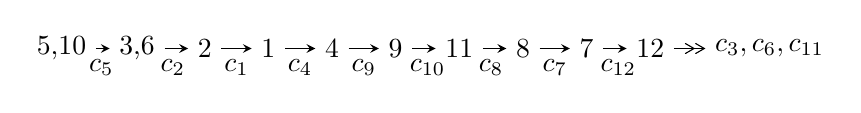
\begin{tikzpicture}[x=23pt, y=7pt]
	% node
	\node (A0) at (-1/8, 0) {5,10};
	\node (A1) at (17/16, 0) {3,6};
	\node (A2) at (17/8, 0) {2};
	\node (A3) at (25/8, 0) {1};
	\node (A4) at (33/8, 0) {4};
	\node (A5) at (41/8, 0) {9};
	\node (A6) at (49/8, 0) {11};
	\node (A7) at (57/8, 0) {8};
	\node (A8) at (65/8, 0) {7};
	\node (A9) at (73/8, 0) {12};
	\node (C1) at (1/2, -1) {$c_{5}$};
	\node (C2) at (13/8, -1) {$c_{2}$};
	\node (C3) at (21/8, -1) {$c_{1}$};
	\node (C4) at (29/8, -1) {$c_{4}$};
	\node (C5) at (37/8, -1) {$c_{9}$};
	\node (C6) at (45/8, -1) {$c_{10}$};
	\node (C7) at (53/8, -1) {$c_{8}$};
	\node (C8) at (61/8, -1) {$c_{7}$};
	\node (C9) at (69/8, -1) {$c_{12}$};
	\node (A10) at (11, 0) {$c_{3},c_{6},c_{11}$};

	% edge
	\draw[->,>=stealth]	
	(A0) edge (A1) (A1) edge (A2) (A2) edge (A3) (A3) edge (A4) (A4) edge (A5) (A5) edge (A6) (A6) edge (A7) (A7) edge (A8) (A8) edge (A9) ;
	\draw[->>,>={angle 60}]	
	(A9) edge (A10);
\end{tikzpicture} \\ 

\end{tabular} \\

\footnotetext{
The image of knot diagram is generated by the software ``\textbf{Draw programme}" developed by Andrew Bartholomew(\url{http://www.layer8.co.uk/maths/draw/index.htm\#Running-draw}), where we modified some parts for our purpose(\url{https://github.com/CATsTAILs/LinksPainter}).
}\phantom \\ \newline 
\centering \textbf{Ideals for irreducible components\footnotemark of $X_{\text{par}}$} 
 
\begin{align*}
I^u_{1}&=\langle 
-4.91771\times10^{36} u^{41}-1.79820\times10^{38} u^{40}+\cdots+2.88772\times10^{39} b+4.22720\times10^{39},\\
\phantom{I^u_{1}}&\phantom{= \langle  }9.16076\times10^{39} u^{41}-6.73128\times10^{39} u^{40}+\cdots+4.90913\times10^{40} a+8.21058\times10^{40},\;u^{42}-2 u^{41}+\cdots+16 u-17\rangle \\
I^u_{2}&=\langle 
b+1,\;-2 u^8+u^7+5 u^6-3 u^5-4 u^4+3 u^3-2 u^2+a+2,\;u^9- u^8-2 u^7+3 u^6+u^5-3 u^4+2 u^3- u+1\rangle \\
I^u_{3}&=\langle 
33 u^3 a^2-5 a^2 u^2-4 u^3 a-30 a^2 u+106 u^2 a+89 u^3-19 a^2+7 a u+28 u^2+185 b-19 a-54 u-160,\\
\phantom{I^u_{3}}&\phantom{= \langle  }- a^2 u^2-5 u^3 a+a^3+3 a^2 u+4 u^2 a- a^2+4 a u+6 u^2- a- u+1,\;u^4- u^2+1\rangle \\
\\
\end{align*}
\raggedright * 3 irreducible components of $\dim_{\mathbb{C}}=0$, with total 63 representations.\\
\footnotetext{All coefficients of polynomials are rational numbers. But the coefficients are sometimes approximated in decimal forms when there is not enough margin.}
\newpage
\renewcommand{\arraystretch}{1}
\centering \section*{I. $I^u_{1}= \langle -4.92\times10^{36} u^{41}-1.80\times10^{38} u^{40}+\cdots+2.89\times10^{39} b+4.23\times10^{39},\;9.16\times10^{39} u^{41}-6.73\times10^{39} u^{40}+\cdots+4.91\times10^{40} a+8.21\times10^{40},\;u^{42}-2 u^{41}+\cdots+16 u-17 \rangle$}
\flushleft \textbf{(i) Arc colorings}\\
\begin{tabular}{m{7pt} m{180pt} m{7pt} m{180pt} }
\flushright $a_{5}=$&$\begin{pmatrix}1\\0\end{pmatrix}$ \\
\flushright $a_{10}=$&$\begin{pmatrix}0\\u\end{pmatrix}$ \\
\flushright $a_{3}=$&$\begin{pmatrix}-0.186607 u^{41}+0.137118 u^{40}+\cdots+5.29366 u-1.67251\\0.00170297 u^{41}+0.0622705 u^{40}+\cdots-0.201147 u-1.46385\end{pmatrix}$ \\
\flushright $a_{6}=$&$\begin{pmatrix}1\\- u^2\end{pmatrix}$ \\
\flushright $a_{2}=$&$\begin{pmatrix}-0.184904 u^{41}+0.199388 u^{40}+\cdots+5.09252 u-3.13636\\0.00170297 u^{41}+0.0622705 u^{40}+\cdots-0.201147 u-1.46385\end{pmatrix}$ \\
\flushright $a_{1}=$&$\begin{pmatrix}0.0588482 u^{41}-0.261568 u^{40}+\cdots+3.71273 u+4.22681\\0.266107 u^{41}-0.115441 u^{40}+\cdots-1.21463 u+2.00517\end{pmatrix}$ \\
\flushright $a_{4}=$&$\begin{pmatrix}0.0875371 u^{41}-0.115951 u^{40}+\cdots+5.83351 u+3.00873\\0.0353514 u^{41}-0.0574630 u^{40}+\cdots-0.374380 u-0.0632026\end{pmatrix}$ \\
\flushright $a_{9}=$&$\begin{pmatrix}- u\\u\end{pmatrix}$ \\
\flushright $a_{11}=$&$\begin{pmatrix}u^3\\- u^3+u\end{pmatrix}$ \\
\flushright $a_{8}=$&$\begin{pmatrix}- u^3\\u^5- u^3+u\end{pmatrix}$ \\
\flushright $a_{7}=$&$\begin{pmatrix}-0.596514 u^{41}+0.435647 u^{40}+\cdots+2.54867 u-8.20884\\0.687055 u^{41}-0.666732 u^{40}+\cdots-0.496210 u+10.8635\end{pmatrix}$ \\
\flushright $a_{12}=$&$\begin{pmatrix}0.589024 u^{41}-0.658891 u^{40}+\cdots+2.42549 u+11.2674\\0.0500035 u^{41}+0.0678910 u^{40}+\cdots-1.20598 u-1.53919\end{pmatrix}$\\&\end{tabular}
\flushleft \textbf{(ii) Obstruction class $= -1$}\\~\\
\flushleft \textbf{(iii) Cusp Shapes $= 1.57605 u^{41}-2.80061 u^{40}+\cdots+23.4107 u+46.2988$}\\~\\
\newpage\renewcommand{\arraystretch}{1}
\flushleft \textbf{(iv) u-Polynomials at the component}\newline \\
\begin{tabular}{m{50pt}|m{274pt}}
Crossings & \hspace{64pt}u-Polynomials at each crossing \\
\hline $$\begin{aligned}c_{1}\end{aligned}$$&$\begin{aligned}
&u^{42}+2 u^{41}+\cdots+24 u+1
\end{aligned}$\\
\hline $$\begin{aligned}c_{2},c_{4}\end{aligned}$$&$\begin{aligned}
&u^{42}-14 u^{41}+\cdots+12 u-1
\end{aligned}$\\
\hline $$\begin{aligned}c_{3},c_{7}\end{aligned}$$&$\begin{aligned}
&u^{42}- u^{41}+\cdots+5632 u+512
\end{aligned}$\\
\hline $$\begin{aligned}c_{5},c_{9}\end{aligned}$$&$\begin{aligned}
&u^{42}-2 u^{41}+\cdots+16 u-17
\end{aligned}$\\
\hline $$\begin{aligned}c_{6},c_{11}\end{aligned}$$&$\begin{aligned}
&u^{42}-2 u^{41}+\cdots-70 u-49
\end{aligned}$\\
\hline $$\begin{aligned}c_{8}\end{aligned}$$&$\begin{aligned}
&u^{42}-6 u^{41}+\cdots-2688 u+2567
\end{aligned}$\\
\hline $$\begin{aligned}c_{10}\end{aligned}$$&$\begin{aligned}
&u^{42}-28 u^{41}+\cdots+1206 u+289
\end{aligned}$\\
\hline $$\begin{aligned}c_{12}\end{aligned}$$&$\begin{aligned}
&u^{42}+6 u^{41}+\cdots+26460 u+2401
\end{aligned}$\\
\hline
\end{tabular}\\~\\
\newpage\renewcommand{\arraystretch}{1}
\flushleft \textbf{(v) Riley Polynomials at the component}\newline \\
\begin{tabular}{m{50pt}|m{274pt}}
Crossings & \hspace{64pt}Riley Polynomials at each crossing \\
\hline $$\begin{aligned}c_{1}\end{aligned}$$&$\begin{aligned}
&y^{42}+90 y^{41}+\cdots+1420 y+1
\end{aligned}$\\
\hline $$\begin{aligned}c_{2},c_{4}\end{aligned}$$&$\begin{aligned}
&y^{42}-2 y^{41}+\cdots-24 y+1
\end{aligned}$\\
\hline $$\begin{aligned}c_{3},c_{7}\end{aligned}$$&$\begin{aligned}
&y^{42}-69 y^{41}+\cdots-17301504 y+262144
\end{aligned}$\\
\hline $$\begin{aligned}c_{5},c_{9}\end{aligned}$$&$\begin{aligned}
&y^{42}-28 y^{41}+\cdots+1206 y+289
\end{aligned}$\\
\hline $$\begin{aligned}c_{6},c_{11}\end{aligned}$$&$\begin{aligned}
&y^{42}+6 y^{41}+\cdots+26460 y+2401
\end{aligned}$\\
\hline $$\begin{aligned}c_{8}\end{aligned}$$&$\begin{aligned}
&y^{42}+68 y^{41}+\cdots+1240622 y+6589489
\end{aligned}$\\
\hline $$\begin{aligned}c_{10}\end{aligned}$$&$\begin{aligned}
&y^{42}-20 y^{41}+\cdots-5069826 y+83521
\end{aligned}$\\
\hline $$\begin{aligned}c_{12}\end{aligned}$$&$\begin{aligned}
&y^{42}+74 y^{41}+\cdots-29647548 y+5764801
\end{aligned}$\\
\hline
\end{tabular}\\~\\
\newpage\flushleft \textbf{(vi) Complex Volumes and Cusp Shapes}
$$\begin{array}{c|c|c}  
\text{Solutions to }I^u_{1}& \I (\text{vol} + \sqrt{-1}CS) & \text{Cusp shape}\\
 \hline 
\begin{aligned}
u &= -0.961799 + 0.311389 I \\
a &= \phantom{-}2.02690 - 2.18124 I \\
b &= -0.464784 + 0.408421 I\end{aligned}
 & -1.72797 - 1.37637 I & \phantom{-}4.55612 - 0.38965 I \\ \hline\begin{aligned}
u &= -0.961799 - 0.311389 I \\
a &= \phantom{-}2.02690 + 2.18124 I \\
b &= -0.464784 - 0.408421 I\end{aligned}
 & -1.72797 + 1.37637 I & \phantom{-}4.55612 + 0.38965 I \\ \hline\begin{aligned}
u &= -0.829534 + 0.589200 I \\
a &= \phantom{-}0.947623 + 0.399065 I \\
b &= -0.343165 - 0.102736 I\end{aligned}
 & -1.74074 - 2.33828 I & \phantom{-}4.84594 + 5.31700 I \\ \hline\begin{aligned}
u &= -0.829534 - 0.589200 I \\
a &= \phantom{-}0.947623 - 0.399065 I \\
b &= -0.343165 + 0.102736 I\end{aligned}
 & -1.74074 + 2.33828 I & \phantom{-}4.84594 - 5.31700 I \\ \hline\begin{aligned}
u &= \phantom{-}0.944203 + 0.228207 I \\
a &= -0.16949 + 2.29855 I \\
b &= \phantom{-}0.993256 - 0.666835 I\end{aligned}
 & \phantom{-}2.48881 + 3.70265 I & \phantom{-}6.29949 - 2.05838 I \\ \hline\begin{aligned}
u &= \phantom{-}0.944203 - 0.228207 I \\
a &= -0.16949 - 2.29855 I \\
b &= \phantom{-}0.993256 + 0.666835 I\end{aligned}
 & \phantom{-}2.48881 - 3.70265 I & \phantom{-}6.29949 + 2.05838 I \\ \hline\begin{aligned}
u &= \phantom{-}0.835994 + 0.489683 I \\
a &= -3.35442 + 8.86991 I \\
b &= -1.016890 + 0.004699 I\end{aligned}
 & -3.34089 + 2.03680 I & \phantom{-}95.8127 + 26.5459 I \\ \hline\begin{aligned}
u &= \phantom{-}0.835994 - 0.489683 I \\
a &= -3.35442 - 8.86991 I \\
b &= -1.016890 - 0.004699 I\end{aligned}
 & -3.34089 - 2.03680 I & \phantom{-}95.8127 - 26.5459 I \\ \hline\begin{aligned}
u &= \phantom{-}0.965269 + 0.439008 I \\
a &= -0.983823 - 0.359781 I \\
b &= \phantom{-}0.899894 + 0.651256 I\end{aligned}
 & \phantom{-}2.81421 - 1.00795 I & \phantom{-}8.57321 + 1.27913 I \\ \hline\begin{aligned}
u &= \phantom{-}0.965269 - 0.439008 I \\
a &= -0.983823 + 0.359781 I \\
b &= \phantom{-}0.899894 - 0.651256 I\end{aligned}
 & \phantom{-}2.81421 + 1.00795 I & \phantom{-}8.57321 - 1.27913 I\\
 \hline 
 \end{array}$$\newpage$$\begin{array}{c|c|c}  
\text{Solutions to }I^u_{1}& \I (\text{vol} + \sqrt{-1}CS) & \text{Cusp shape}\\
 \hline 
\begin{aligned}
u &= -0.726987 + 0.560951 I \\
a &= \phantom{-}0.802280 + 0.067898 I \\
b &= \phantom{-}0.101623 + 0.134205 I\end{aligned}
 & -1.85016 - 2.19168 I & \phantom{-}2.73443 + 3.94919 I \\ \hline\begin{aligned}
u &= -0.726987 - 0.560951 I \\
a &= \phantom{-}0.802280 - 0.067898 I \\
b &= \phantom{-}0.101623 - 0.134205 I\end{aligned}
 & -1.85016 + 2.19168 I & \phantom{-}2.73443 - 3.94919 I \\ \hline\begin{aligned}
u &= \phantom{-}0.205294 + 1.093670 I \\
a &= -0.50667 - 1.38304 I \\
b &= \phantom{-}1.23869 + 1.08212 I\end{aligned}
 & \phantom{-}11.4259 - 8.4418 I & \phantom{-}2.24860 + 3.75985 I \\ \hline\begin{aligned}
u &= \phantom{-}0.205294 - 1.093670 I \\
a &= -0.50667 + 1.38304 I \\
b &= \phantom{-}1.23869 - 1.08212 I\end{aligned}
 & \phantom{-}11.4259 + 8.4418 I & \phantom{-}2.24860 - 3.75985 I \\ \hline\begin{aligned}
u &= \phantom{-}0.053594 + 1.137510 I \\
a &= -0.59511 + 1.46169 I \\
b &= \phantom{-}1.05760 - 1.28040 I\end{aligned}
 & \phantom{-}12.15940 + 0.20639 I & \phantom{-}3.10494 - 0.07106 I \\ \hline\begin{aligned}
u &= \phantom{-}0.053594 - 1.137510 I \\
a &= -0.59511 - 1.46169 I \\
b &= \phantom{-}1.05760 + 1.28040 I\end{aligned}
 & \phantom{-}12.15940 - 0.20639 I & \phantom{-}3.10494 + 0.07106 I \\ \hline\begin{aligned}
u &= \phantom{-}0.232942 + 0.816588 I \\
a &= \phantom{-}0.184697 - 0.861641 I \\
b &= \phantom{-}0.151638 + 0.884654 I\end{aligned}
 & \phantom{-}1.95152 + 0.96411 I & \phantom{-}4.49813 - 1.84965 I \\ \hline\begin{aligned}
u &= \phantom{-}0.232942 - 0.816588 I \\
a &= \phantom{-}0.184697 + 0.861641 I \\
b &= \phantom{-}0.151638 - 0.884654 I\end{aligned}
 & \phantom{-}1.95152 - 0.96411 I & \phantom{-}4.49813 + 1.84965 I \\ \hline\begin{aligned}
u &= -1.18461\phantom{ +0.000000I} \\
a &= \phantom{-}1.51253\phantom{ +0.000000I} \\
b &= -1.40973\phantom{ +0.000000I}\end{aligned}
 & \phantom{-}0.934538\phantom{ +0.000000I} & \phantom{-}7.24150\phantom{ +0.000000I} \\ \hline\begin{aligned}
u &= -1.126130 + 0.490429 I \\
a &= -0.039913 - 1.285050 I \\
b &= \phantom{-}0.828323 + 0.354167 I\end{aligned}
 & \phantom{-}2.33209 - 7.91667 I & \phantom{-}6.88839 + 11.06602 I\\
 \hline 
 \end{array}$$\newpage$$\begin{array}{c|c|c}  
\text{Solutions to }I^u_{1}& \I (\text{vol} + \sqrt{-1}CS) & \text{Cusp shape}\\
 \hline 
\begin{aligned}
u &= -1.126130 - 0.490429 I \\
a &= -0.039913 + 1.285050 I \\
b &= \phantom{-}0.828323 - 0.354167 I\end{aligned}
 & \phantom{-}2.33209 + 7.91667 I & \phantom{-}6.88839 - 11.06602 I \\ \hline\begin{aligned}
u &= \phantom{-}1.259460 + 0.006196 I \\
a &= -0.97423 - 2.37844 I \\
b &= \phantom{-}0.506833 + 1.138780 I\end{aligned}
 & \phantom{-}4.47907 - 1.92884 I & \phantom{-}6.47929 + 1.71581 I \\ \hline\begin{aligned}
u &= \phantom{-}1.259460 - 0.006196 I \\
a &= -0.97423 + 2.37844 I \\
b &= \phantom{-}0.506833 - 1.138780 I\end{aligned}
 & \phantom{-}4.47907 + 1.92884 I & \phantom{-}6.47929 - 1.71581 I \\ \hline\begin{aligned}
u &= \phantom{-}1.072950 + 0.670917 I \\
a &= \phantom{-}0.45051 + 1.91983 I \\
b &= \phantom{-}0.590513 - 1.035150 I\end{aligned}
 & \phantom{-}4.15910 + 4.29767 I & \phantom{-}6.40450 - 3.97494 I \\ \hline\begin{aligned}
u &= \phantom{-}1.072950 - 0.670917 I \\
a &= \phantom{-}0.45051 - 1.91983 I \\
b &= \phantom{-}0.590513 + 1.035150 I\end{aligned}
 & \phantom{-}4.15910 - 4.29767 I & \phantom{-}6.40450 + 3.97494 I \\ \hline\begin{aligned}
u &= \phantom{-}1.254550 + 0.204489 I \\
a &= \phantom{-}1.39168 - 2.27514 I \\
b &= -1.145780 + 0.655072 I\end{aligned}
 & \phantom{-}2.23820 + 2.99548 I & \phantom{-}5.68648 - 2.96480 I \\ \hline\begin{aligned}
u &= \phantom{-}1.254550 - 0.204489 I \\
a &= \phantom{-}1.39168 + 2.27514 I \\
b &= -1.145780 - 0.655072 I\end{aligned}
 & \phantom{-}2.23820 - 2.99548 I & \phantom{-}5.68648 + 2.96480 I \\ \hline\begin{aligned}
u &= -0.274846 + 0.651125 I \\
a &= \phantom{-}0.435590 + 0.051488 I \\
b &= \phantom{-}0.661252 - 0.443712 I\end{aligned}
 & -0.15519 + 3.49196 I & \phantom{-}2.75035 - 5.76254 I \\ \hline\begin{aligned}
u &= -0.274846 - 0.651125 I \\
a &= \phantom{-}0.435590 - 0.051488 I \\
b &= \phantom{-}0.661252 + 0.443712 I\end{aligned}
 & -0.15519 - 3.49196 I & \phantom{-}2.75035 + 5.76254 I \\ \hline\begin{aligned}
u &= \phantom{-}0.698771\phantom{ +0.000000I} \\
a &= \phantom{-}0.544644\phantom{ +0.000000I} \\
b &= \phantom{-}0.196513\phantom{ +0.000000I}\end{aligned}
 & \phantom{-}0.929263\phantom{ +0.000000I} & \phantom{-}11.4390\phantom{ +0.000000I}\\
 \hline 
 \end{array}$$\newpage$$\begin{array}{c|c|c}  
\text{Solutions to }I^u_{1}& \I (\text{vol} + \sqrt{-1}CS) & \text{Cusp shape}\\
 \hline 
\begin{aligned}
u &= -1.360000 + 0.378690 I \\
a &= -0.10332 + 2.56500 I \\
b &= -0.202310 - 1.252300 I\end{aligned}
 & \phantom{-}6.81382 - 5.26231 I & \phantom{-0.000000 } 0 \\ \hline\begin{aligned}
u &= -1.360000 - 0.378690 I \\
a &= -0.10332 - 2.56500 I \\
b &= -0.202310 + 1.252300 I\end{aligned}
 & \phantom{-}6.81382 + 5.26231 I & \phantom{-0.000000 } 0 \\ \hline\begin{aligned}
u &= \phantom{-}1.29496 + 0.63382 I \\
a &= -0.59935 + 2.83045 I \\
b &= \phantom{-}1.31294 - 0.99932 I\end{aligned}
 & \phantom{-}14.7912 + 14.5915 I & \phantom{-0.000000 } 0 \\ \hline\begin{aligned}
u &= \phantom{-}1.29496 - 0.63382 I \\
a &= -0.59935 - 2.83045 I \\
b &= \phantom{-}1.31294 + 0.99932 I\end{aligned}
 & \phantom{-}14.7912 - 14.5915 I & \phantom{-0.000000 } 0 \\ \hline\begin{aligned}
u &= \phantom{-}1.38494 + 0.58465 I \\
a &= -1.93831 - 1.93197 I \\
b &= \phantom{-}0.92670 + 1.41166 I\end{aligned}
 & \phantom{-}16.3124 + 5.9260 I & \phantom{-0.000000 } 0 \\ \hline\begin{aligned}
u &= \phantom{-}1.38494 - 0.58465 I \\
a &= -1.93831 + 1.93197 I \\
b &= \phantom{-}0.92670 - 1.41166 I\end{aligned}
 & \phantom{-}16.3124 - 5.9260 I & \phantom{-0.000000 } 0 \\ \hline\begin{aligned}
u &= -1.42037 + 0.52003 I \\
a &= -0.95320 - 2.91761 I \\
b &= \phantom{-}1.24919 + 1.24050 I\end{aligned}
 & \phantom{-}16.8335 - 6.1018 I & \phantom{-0.000000 } 0 \\ \hline\begin{aligned}
u &= -1.42037 - 0.52003 I \\
a &= -0.95320 + 2.91761 I \\
b &= \phantom{-}1.24919 - 1.24050 I\end{aligned}
 & \phantom{-}16.8335 + 6.1018 I & \phantom{-0.000000 } 0 \\ \hline\begin{aligned}
u &= -1.46489 + 0.38079 I \\
a &= -2.05057 + 2.08335 I \\
b &= \phantom{-}1.22965 - 1.27108 I\end{aligned}
 & \phantom{-}16.9282 + 3.1689 I & \phantom{-0.000000 } 0 \\ \hline\begin{aligned}
u &= -1.46489 - 0.38079 I \\
a &= -2.05057 - 2.08335 I \\
b &= \phantom{-}1.22965 + 1.27108 I\end{aligned}
 & \phantom{-}16.9282 - 3.1689 I & \phantom{-0.000000 } 0\\
 \hline 
 \end{array}$$\newpage$$\begin{array}{c|c|c}  
\text{Solutions to }I^u_{1}& \I (\text{vol} + \sqrt{-1}CS) & \text{Cusp shape}\\
 \hline 
\begin{aligned}
u &= -0.096688 + 0.349533 I \\
a &= -0.82299 + 1.83040 I \\
b &= -0.968549 - 0.219170 I\end{aligned}
 & -1.74611 - 0.73385 I & -3.54446 + 0.56735 I \\ \hline\begin{aligned}
u &= -0.096688 - 0.349533 I \\
a &= -0.82299 - 1.83040 I \\
b &= -0.968549 + 0.219170 I\end{aligned}
 & -1.74611 + 0.73385 I & -3.54446 - 0.56735 I\\
 \hline 
 \end{array}$$\newpage\newpage\renewcommand{\arraystretch}{1}
\centering \section*{II. $I^u_{2}= \langle b+1,\;-2 u^8+u^7+\cdots+a+2,\;u^9- u^8-2 u^7+3 u^6+u^5-3 u^4+2 u^3- u+1 \rangle$}
\flushleft \textbf{(i) Arc colorings}\\
\begin{tabular}{m{7pt} m{180pt} m{7pt} m{180pt} }
\flushright $a_{5}=$&$\begin{pmatrix}1\\0\end{pmatrix}$ \\
\flushright $a_{10}=$&$\begin{pmatrix}0\\u\end{pmatrix}$ \\
\flushright $a_{3}=$&$\begin{pmatrix}2 u^8- u^7-5 u^6+3 u^5+4 u^4-3 u^3+2 u^2-2\\-1\end{pmatrix}$ \\
\flushright $a_{6}=$&$\begin{pmatrix}1\\- u^2\end{pmatrix}$ \\
\flushright $a_{2}=$&$\begin{pmatrix}2 u^8- u^7-5 u^6+3 u^5+4 u^4-3 u^3+2 u^2-3\\-1\end{pmatrix}$ \\
\flushright $a_{1}=$&$\begin{pmatrix}-1\\0\end{pmatrix}$ \\
\flushright $a_{4}=$&$\begin{pmatrix}2 u^8- u^7-5 u^6+3 u^5+4 u^4-3 u^3+2 u^2-2\\-1\end{pmatrix}$ \\
\flushright $a_{9}=$&$\begin{pmatrix}- u\\u\end{pmatrix}$ \\
\flushright $a_{11}=$&$\begin{pmatrix}u^3\\- u^3+u\end{pmatrix}$ \\
\flushright $a_{8}=$&$\begin{pmatrix}- u^3\\u^5- u^3+u\end{pmatrix}$ \\
\flushright $a_{7}=$&$\begin{pmatrix}- u^3\\u^5- u^3+u\end{pmatrix}$ \\
\flushright $a_{12}=$&$\begin{pmatrix}- u^6+u^4-1\\u^6-2 u^4+u^2\end{pmatrix}$\\&\end{tabular}
\flushleft \textbf{(ii) Obstruction class $= 1$}\\~\\
\flushleft \textbf{(iii) Cusp Shapes $= -6 u^8-5 u^7+10 u^6+8 u^5-10 u^4-8 u^3-4 u^2-8 u-2$}\\~\\
\newpage\renewcommand{\arraystretch}{1}
\flushleft \textbf{(iv) u-Polynomials at the component}\newline \\
\begin{tabular}{m{50pt}|m{274pt}}
Crossings & \hspace{64pt}u-Polynomials at each crossing \\
\hline $$\begin{aligned}c_{1},c_{2}\end{aligned}$$&$\begin{aligned}
&(u-1)^9
\end{aligned}$\\
\hline $$\begin{aligned}c_{3},c_{7}\end{aligned}$$&$\begin{aligned}
&u^9
\end{aligned}$\\
\hline $$\begin{aligned}c_{4}\end{aligned}$$&$\begin{aligned}
&(u+1)^9
\end{aligned}$\\
\hline $$\begin{aligned}c_{5}\end{aligned}$$&$\begin{aligned}
&u^9- u^8-2 u^7+3 u^6+u^5-3 u^4+2 u^3- u+1
\end{aligned}$\\
\hline $$\begin{aligned}c_{6}\end{aligned}$$&$\begin{aligned}
&u^9- u^8+2 u^7- u^6+3 u^5- u^4+2 u^3+u+1
\end{aligned}$\\
\hline $$\begin{aligned}c_{8},c_{12}\end{aligned}$$&$\begin{aligned}
&u^9+3 u^8+8 u^7+13 u^6+17 u^5+17 u^4+12 u^3+6 u^2+u-1
\end{aligned}$\\
\hline $$\begin{aligned}c_{9}\end{aligned}$$&$\begin{aligned}
&u^9+u^8-2 u^7-3 u^6+u^5+3 u^4+2 u^3- u-1
\end{aligned}$\\
\hline $$\begin{aligned}c_{10}\end{aligned}$$&$\begin{aligned}
&u^9-5 u^8+12 u^7-15 u^6+9 u^5+u^4-4 u^3+2 u^2+u-1
\end{aligned}$\\
\hline $$\begin{aligned}c_{11}\end{aligned}$$&$\begin{aligned}
&u^9+u^8+2 u^7+u^6+3 u^5+u^4+2 u^3+u-1
\end{aligned}$\\
\hline
\end{tabular}\\~\\
\newpage\renewcommand{\arraystretch}{1}
\flushleft \textbf{(v) Riley Polynomials at the component}\newline \\
\begin{tabular}{m{50pt}|m{274pt}}
Crossings & \hspace{64pt}Riley Polynomials at each crossing \\
\hline $$\begin{aligned}c_{1},c_{2},c_{4}\end{aligned}$$&$\begin{aligned}
&(y-1)^9
\end{aligned}$\\
\hline $$\begin{aligned}c_{3},c_{7}\end{aligned}$$&$\begin{aligned}
&y^9
\end{aligned}$\\
\hline $$\begin{aligned}c_{5},c_{9}\end{aligned}$$&$\begin{aligned}
&y^9-5 y^8+12 y^7-15 y^6+9 y^5+y^4-4 y^3+2 y^2+y-1
\end{aligned}$\\
\hline $$\begin{aligned}c_{6},c_{11}\end{aligned}$$&$\begin{aligned}
&y^9+3 y^8+8 y^7+13 y^6+17 y^5+17 y^4+12 y^3+6 y^2+y-1
\end{aligned}$\\
\hline $$\begin{aligned}c_{8},c_{12}\end{aligned}$$&$\begin{aligned}
&y^9+7 y^8+20 y^7+25 y^6+5 y^5-15 y^4+22 y^2+13 y-1
\end{aligned}$\\
\hline $$\begin{aligned}c_{10}\end{aligned}$$&$\begin{aligned}
&y^9- y^8+12 y^7-7 y^6+37 y^5+y^4-10 y^2+5 y-1
\end{aligned}$\\
\hline
\end{tabular}\\~\\
\newpage\flushleft \textbf{(vi) Complex Volumes and Cusp Shapes}
$$\begin{array}{c|c|c}  
\text{Solutions to }I^u_{2}& \I (\text{vol} + \sqrt{-1}CS) & \text{Cusp shape}\\
 \hline 
\begin{aligned}
u &= \phantom{-}0.772920 + 0.510351 I \\
a &= -1.67861 + 2.31573 I \\
b &= -1.00000\phantom{ +0.000000I}\end{aligned}
 & -3.42837 + 2.09337 I & -12.6725 - 14.2088 I \\ \hline\begin{aligned}
u &= \phantom{-}0.772920 - 0.510351 I \\
a &= -1.67861 - 2.31573 I \\
b &= -1.00000\phantom{ +0.000000I}\end{aligned}
 & -3.42837 - 2.09337 I & -12.6725 + 14.2088 I \\ \hline\begin{aligned}
u &= -0.825933\phantom{ +0.000000I} \\
a &= \phantom{-}0.871015\phantom{ +0.000000I} \\
b &= -1.00000\phantom{ +0.000000I}\end{aligned}
 & -0.446489\phantom{ +0.000000I} & \phantom{-}1.84400\phantom{ +0.000000I} \\ \hline\begin{aligned}
u &= -1.173910 + 0.391555 I \\
a &= \phantom{-}0.893484 + 0.630694 I \\
b &= -1.00000\phantom{ +0.000000I}\end{aligned}
 & \phantom{-}2.72642 - 1.33617 I & \phantom{-}6.61905 + 0.64999 I \\ \hline\begin{aligned}
u &= -1.173910 - 0.391555 I \\
a &= \phantom{-}0.893484 - 0.630694 I \\
b &= -1.00000\phantom{ +0.000000I}\end{aligned}
 & \phantom{-}2.72642 + 1.33617 I & \phantom{-}6.61905 - 0.64999 I \\ \hline\begin{aligned}
u &= \phantom{-}0.141484 + 0.739668 I \\
a &= -0.309843 + 0.043204 I \\
b &= -1.00000\phantom{ +0.000000I}\end{aligned}
 & -1.02799 - 2.45442 I & -0.10038 + 1.90984 I \\ \hline\begin{aligned}
u &= \phantom{-}0.141484 - 0.739668 I \\
a &= -0.309843 - 0.043204 I \\
b &= -1.00000\phantom{ +0.000000I}\end{aligned}
 & -1.02799 + 2.45442 I & -0.10038 - 1.90984 I \\ \hline\begin{aligned}
u &= \phantom{-}1.172470 + 0.500383 I \\
a &= \phantom{-}0.659464 - 0.874093 I \\
b &= -1.00000\phantom{ +0.000000I}\end{aligned}
 & \phantom{-}1.95319 + 7.08493 I & \phantom{-}3.23178 - 2.93209 I \\ \hline\begin{aligned}
u &= \phantom{-}1.172470 - 0.500383 I \\
a &= \phantom{-}0.659464 + 0.874093 I \\
b &= -1.00000\phantom{ +0.000000I}\end{aligned}
 & \phantom{-}1.95319 - 7.08493 I & \phantom{-}3.23178 + 2.93209 I\\
 \hline 
 \end{array}$$\newpage\newpage\renewcommand{\arraystretch}{1}
\centering \section*{III. $I^u_{3}= \langle 33 u^3 a^2-4 u^3 a+\cdots-19 a-160,\;- a^2 u^2-5 u^3 a+\cdots- a+1,\;u^4- u^2+1 \rangle$}
\flushleft \textbf{(i) Arc colorings}\\
\begin{tabular}{m{7pt} m{180pt} m{7pt} m{180pt} }
\flushright $a_{5}=$&$\begin{pmatrix}1\\0\end{pmatrix}$ \\
\flushright $a_{10}=$&$\begin{pmatrix}0\\u\end{pmatrix}$ \\
\flushright $a_{3}=$&$\begin{pmatrix}a\\-0.178378 a^{2} u^{3}+0.0216216 a u^{3}+\cdots+0.102703 a+0.864865\end{pmatrix}$ \\
\flushright $a_{6}=$&$\begin{pmatrix}1\\- u^2\end{pmatrix}$ \\
\flushright $a_{2}=$&$\begin{pmatrix}-0.178378 a^{2} u^{3}+0.0216216 a u^{3}+\cdots+1.10270 a+0.864865\\-0.178378 a^{2} u^{3}+0.0216216 a u^{3}+\cdots+0.102703 a+0.864865\end{pmatrix}$ \\
\flushright $a_{1}=$&$\begin{pmatrix}0.156757 a^{2} u^{3}-0.0432432 a u^{3}+\cdots-0.00540541 a-1.32973\\-0.232432 a^{2} u^{3}-0.632432 a u^{3}+\cdots-0.0540541 a+2.10270\end{pmatrix}$ \\
\flushright $a_{4}=$&$\begin{pmatrix}\frac{1}{5} u^3 a^2-\frac{3}{5} u^3 a+\cdots-\frac{3}{5} a+1\\-0.0540541 a^{2} u^{3}-0.654054 a u^{3}+\cdots-0.156757 a+0.237838\end{pmatrix}$ \\
\flushright $a_{9}=$&$\begin{pmatrix}- u\\u\end{pmatrix}$ \\
\flushright $a_{11}=$&$\begin{pmatrix}u^3\\- u^3+u\end{pmatrix}$ \\
\flushright $a_{8}=$&$\begin{pmatrix}- u^3\\0\end{pmatrix}$ \\
\flushright $a_{7}=$&$\begin{pmatrix}0.340541 a^{2} u^{3}-0.0594595 a u^{3}+\cdots-0.632432 a+0.421622\\-0.194595 a^{2} u^{3}+0.00540541 a u^{3}+\cdots+0.675676 a+1.01622\end{pmatrix}$ \\
\flushright $a_{12}=$&$\begin{pmatrix}0.156757 a^{2} u^{3}-0.0432432 a u^{3}+\cdots-0.00540541 a-1.32973\\-0.232432 a^{2} u^{3}-0.632432 a u^{3}+\cdots-0.0540541 a+2.10270\end{pmatrix}$\\&\end{tabular}
\flushleft \textbf{(ii) Obstruction class $= 1$}\\~\\
\flushleft \textbf{(iii) Cusp Shapes $= -\frac{132}{185} u^3 a^2+\frac{4}{37} a^2 u^2+\frac{16}{185} u^3 a+\frac{24}{37} a^2 u-\frac{424}{185} u^2 a-\frac{356}{185} u^3+\frac{76}{185} a^2-\frac{28}{185} a u-\frac{852}{185} u^2+\frac{76}{185} a+\frac{216}{185} u+\frac{128}{37}$}\\~\\
\newpage\renewcommand{\arraystretch}{1}
\flushleft \textbf{(iv) u-Polynomials at the component}\newline \\
\begin{tabular}{m{50pt}|m{274pt}}
Crossings & \hspace{64pt}u-Polynomials at each crossing \\
\hline $$\begin{aligned}c_{1}\end{aligned}$$&$\begin{aligned}
&(u^3- u^2+2 u-1)^4
\end{aligned}$\\
\hline $$\begin{aligned}c_{2}\end{aligned}$$&$\begin{aligned}
&(u^3+u^2-1)^4
\end{aligned}$\\
\hline $$\begin{aligned}c_{3},c_{7}\end{aligned}$$&$\begin{aligned}
&(u^6-3 u^4+2 u^2+1)^2
\end{aligned}$\\
\hline $$\begin{aligned}c_{4}\end{aligned}$$&$\begin{aligned}
&(u^3- u^2+1)^4
\end{aligned}$\\
\hline $$\begin{aligned}c_{5},c_{8},c_{9}\end{aligned}$$&$\begin{aligned}
&(u^4- u^2+1)^3
\end{aligned}$\\
\hline $$\begin{aligned}c_{6},c_{11}\end{aligned}$$&$\begin{aligned}
&(u^2+1)^6
\end{aligned}$\\
\hline $$\begin{aligned}c_{10}\end{aligned}$$&$\begin{aligned}
&(u^2- u+1)^6
\end{aligned}$\\
\hline $$\begin{aligned}c_{12}\end{aligned}$$&$\begin{aligned}
&(u+1)^{12}
\end{aligned}$\\
\hline
\end{tabular}\\~\\
\newpage\renewcommand{\arraystretch}{1}
\flushleft \textbf{(v) Riley Polynomials at the component}\newline \\
\begin{tabular}{m{50pt}|m{274pt}}
Crossings & \hspace{64pt}Riley Polynomials at each crossing \\
\hline $$\begin{aligned}c_{1}\end{aligned}$$&$\begin{aligned}
&(y^3+3 y^2+2 y-1)^4
\end{aligned}$\\
\hline $$\begin{aligned}c_{2},c_{4}\end{aligned}$$&$\begin{aligned}
&(y^3- y^2+2 y-1)^4
\end{aligned}$\\
\hline $$\begin{aligned}c_{3},c_{7}\end{aligned}$$&$\begin{aligned}
&(y^3-3 y^2+2 y+1)^4
\end{aligned}$\\
\hline $$\begin{aligned}c_{5},c_{8},c_{9}\end{aligned}$$&$\begin{aligned}
&(y^2- y+1)^6
\end{aligned}$\\
\hline $$\begin{aligned}c_{6},c_{11}\end{aligned}$$&$\begin{aligned}
&(y+1)^{12}
\end{aligned}$\\
\hline $$\begin{aligned}c_{10}\end{aligned}$$&$\begin{aligned}
&(y^2+y+1)^6
\end{aligned}$\\
\hline $$\begin{aligned}c_{12}\end{aligned}$$&$\begin{aligned}
&(y-1)^{12}
\end{aligned}$\\
\hline
\end{tabular}\\~\\
\newpage\flushleft \textbf{(vi) Complex Volumes and Cusp Shapes}
$$\begin{array}{c|c|c}  
\text{Solutions to }I^u_{3}& \I (\text{vol} + \sqrt{-1}CS) & \text{Cusp shape}\\
 \hline 
\begin{aligned}
u &= \phantom{-}0.866025 + 0.500000 I \\
a &= -0.972493 - 1.013180 I \\
b &= \phantom{-}0.877439 + 0.744862 I\end{aligned}
 & \phantom{-}1.37919 - 0.79824 I & \phantom{-}1.50976 - 0.48465 I \\ \hline\begin{aligned}
u &= \phantom{-}0.866025 + 0.500000 I \\
a &= \phantom{-}0.11905 - 1.81610 I \\
b &= -0.754878\phantom{ +0.000000I}\end{aligned}
 & -2.75839 + 2.02988 I & -5.01951 - 3.46410 I \\ \hline\begin{aligned}
u &= \phantom{-}0.866025 + 0.500000 I \\
a &= -0.24463 + 2.19530 I \\
b &= \phantom{-}0.877439 - 0.744862 I\end{aligned}
 & \phantom{-}1.37919 + 4.85801 I & \phantom{-}1.50976 - 6.44355 I \\ \hline\begin{aligned}
u &= \phantom{-}0.866025 - 0.500000 I \\
a &= -0.972493 + 1.013180 I \\
b &= \phantom{-}0.877439 - 0.744862 I\end{aligned}
 & \phantom{-}1.37919 + 0.79824 I & \phantom{-}1.50976 + 0.48465 I \\ \hline\begin{aligned}
u &= \phantom{-}0.866025 - 0.500000 I \\
a &= \phantom{-}0.11905 + 1.81610 I \\
b &= -0.754878\phantom{ +0.000000I}\end{aligned}
 & -2.75839 - 2.02988 I & -5.01951 + 3.46410 I \\ \hline\begin{aligned}
u &= \phantom{-}0.866025 - 0.500000 I \\
a &= -0.24463 - 2.19530 I \\
b &= \phantom{-}0.877439 + 0.744862 I\end{aligned}
 & \phantom{-}1.37919 - 4.85801 I & \phantom{-}1.50976 + 6.44355 I \\ \hline\begin{aligned}
u &= -0.866025 + 0.500000 I \\
a &= -0.949962 - 0.298361 I \\
b &= \phantom{-}0.877439 - 0.744862 I\end{aligned}
 & \phantom{-}1.37919 + 0.79824 I & \phantom{-}1.50976 + 0.48465 I \\ \hline\begin{aligned}
u &= -0.866025 + 0.500000 I \\
a &= \phantom{-}0.90246 - 1.55905 I \\
b &= \phantom{-}0.877439 + 0.744862 I\end{aligned}
 & \phantom{-}1.37919 - 4.85801 I & \phantom{-}1.50976 + 6.44355 I \\ \hline\begin{aligned}
u &= -0.866025 + 0.500000 I \\
a &= \phantom{-}4.14558 - 0.50862 I \\
b &= -0.754878\phantom{ +0.000000I}\end{aligned}
 & -2.75839 - 2.02988 I & -5.01951 + 3.46410 I \\ \hline\begin{aligned}
u &= -0.866025 - 0.500000 I \\
a &= -0.949962 + 0.298361 I \\
b &= \phantom{-}0.877439 + 0.744862 I\end{aligned}
 & \phantom{-}1.37919 - 0.79824 I & \phantom{-}1.50976 - 0.48465 I\\
 \hline 
 \end{array}$$\newpage$$\begin{array}{c|c|c}  
\text{Solutions to }I^u_{3}& \I (\text{vol} + \sqrt{-1}CS) & \text{Cusp shape}\\
 \hline 
\begin{aligned}
u &= -0.866025 - 0.500000 I \\
a &= \phantom{-}0.90246 + 1.55905 I \\
b &= \phantom{-}0.877439 - 0.744862 I\end{aligned}
 & \phantom{-}1.37919 + 4.85801 I & \phantom{-}1.50976 - 6.44355 I \\ \hline\begin{aligned}
u &= -0.866025 - 0.500000 I \\
a &= \phantom{-}4.14558 + 0.50862 I \\
b &= -0.754878\phantom{ +0.000000I}\end{aligned}
 & -2.75839 + 2.02988 I & -5.01951 - 3.46410 I\\
 \hline 
 \end{array}$$\newpage
\newpage\renewcommand{\arraystretch}{1}
\centering \section*{ IV. u-Polynomials}
\begin{tabular}{m{50pt}|m{274pt}}
Crossings & \hspace{64pt}u-Polynomials at each crossing \\
\hline $$\begin{aligned}c_{1}\end{aligned}$$&$\begin{aligned}
&((u-1)^9)(u^3- u^2+2 u-1)^4(u^{42}+2 u^{41}+\cdots+24 u+1)
\end{aligned}$\\
\hline $$\begin{aligned}c_{2}\end{aligned}$$&$\begin{aligned}
&((u-1)^9)(u^3+u^2-1)^4(u^{42}-14 u^{41}+\cdots+12 u-1)
\end{aligned}$\\
\hline $$\begin{aligned}c_{3},c_{7}\end{aligned}$$&$\begin{aligned}
&u^9(u^6-3 u^4+2 u^2+1)^2(u^{42}-u^{41}+\cdots+5632 u+512)
\end{aligned}$\\
\hline $$\begin{aligned}c_{4}\end{aligned}$$&$\begin{aligned}
&((u+1)^9)(u^3- u^2+1)^4(u^{42}-14 u^{41}+\cdots+12 u-1)
\end{aligned}$\\
\hline $$\begin{aligned}c_{5}\end{aligned}$$&$\begin{aligned}
&(u^4- u^2+1)^3(u^9- u^8-2 u^7+3 u^6+u^5-3 u^4+2 u^3- u+1)\\
&\cdot(u^{42}-2 u^{41}+\cdots+16 u-17)
\end{aligned}$\\
\hline $$\begin{aligned}c_{6}\end{aligned}$$&$\begin{aligned}
&(u^2+1)^6(u^9- u^8+2 u^7- u^6+3 u^5- u^4+2 u^3+u+1)\\
&\cdot(u^{42}-2 u^{41}+\cdots-70 u-49)
\end{aligned}$\\
\hline $$\begin{aligned}c_{8}\end{aligned}$$&$\begin{aligned}
&(u^4- u^2+1)^3\\
&\cdot(u^9+3 u^8+8 u^7+13 u^6+17 u^5+17 u^4+12 u^3+6 u^2+u-1)\\
&\cdot(u^{42}-6 u^{41}+\cdots-2688 u+2567)
\end{aligned}$\\
\hline $$\begin{aligned}c_{9}\end{aligned}$$&$\begin{aligned}
&(u^4- u^2+1)^3(u^9+u^8-2 u^7-3 u^6+u^5+3 u^4+2 u^3- u-1)\\
&\cdot(u^{42}-2 u^{41}+\cdots+16 u-17)
\end{aligned}$\\
\hline $$\begin{aligned}c_{10}\end{aligned}$$&$\begin{aligned}
&((u^2- u+1)^6)(u^9-5 u^8+\cdots+u-1)\\
&\cdot(u^{42}-28 u^{41}+\cdots+1206 u+289)
\end{aligned}$\\
\hline $$\begin{aligned}c_{11}\end{aligned}$$&$\begin{aligned}
&(u^2+1)^6(u^9+u^8+2 u^7+u^6+3 u^5+u^4+2 u^3+u-1)\\
&\cdot(u^{42}-2 u^{41}+\cdots-70 u-49)
\end{aligned}$\\
\hline $$\begin{aligned}c_{12}\end{aligned}$$&$\begin{aligned}
&((u+1)^{12})(u^9+3 u^8+\cdots+u-1)\\
&\cdot(u^{42}+6 u^{41}+\cdots+26460 u+2401)
\end{aligned}$\\
\hline
\end{tabular}\newpage\renewcommand{\arraystretch}{1}
\centering \section*{ V. Riley Polynomials}
\begin{tabular}{m{50pt}|m{274pt}}
Crossings & \hspace{64pt}Riley Polynomials at each crossing \\
\hline $$\begin{aligned}c_{1}\end{aligned}$$&$\begin{aligned}
&((y-1)^9)(y^3+3 y^2+2 y-1)^4(y^{42}+90 y^{41}+\cdots+1420 y+1)
\end{aligned}$\\
\hline $$\begin{aligned}c_{2},c_{4}\end{aligned}$$&$\begin{aligned}
&((y-1)^9)(y^3- y^2+2 y-1)^4(y^{42}-2 y^{41}+\cdots-24 y+1)
\end{aligned}$\\
\hline $$\begin{aligned}c_{3},c_{7}\end{aligned}$$&$\begin{aligned}
&y^9(y^3-3 y^2+2 y+1)^4(y^{42}-69 y^{41}+\cdots-1.73015\times10^{7} y+262144)
\end{aligned}$\\
\hline $$\begin{aligned}c_{5},c_{9}\end{aligned}$$&$\begin{aligned}
&((y^2- y+1)^6)(y^9-5 y^8+\cdots+y-1)\\
&\cdot(y^{42}-28 y^{41}+\cdots+1206 y+289)
\end{aligned}$\\
\hline $$\begin{aligned}c_{6},c_{11}\end{aligned}$$&$\begin{aligned}
&((y+1)^{12})(y^9+3 y^8+\cdots+y-1)\\
&\cdot(y^{42}+6 y^{41}+\cdots+26460 y+2401)
\end{aligned}$\\
\hline $$\begin{aligned}c_{8}\end{aligned}$$&$\begin{aligned}
&((y^2- y+1)^6)(y^9+7 y^8+\cdots+13 y-1)\\
&\cdot(y^{42}+68 y^{41}+\cdots+1240622 y+6589489)
\end{aligned}$\\
\hline $$\begin{aligned}c_{10}\end{aligned}$$&$\begin{aligned}
&(y^2+y+1)^6(y^9- y^8+12 y^7-7 y^6+37 y^5+y^4-10 y^2+5 y-1)\\
&\cdot(y^{42}-20 y^{41}+\cdots-5069826 y+83521)
\end{aligned}$\\
\hline $$\begin{aligned}c_{12}\end{aligned}$$&$\begin{aligned}
&(y-1)^{12}(y^9+7 y^8+20 y^7+25 y^6+5 y^5-15 y^4+22 y^2+13 y-1)\\
&\cdot(y^{42}+74 y^{41}+\cdots-29647548 y+5764801)
\end{aligned}$\\
\hline
\end{tabular}
\vskip 2pc
\end{document}